\begin{frame}{Challenge de l'ordinateur pour la cryptographie}

  \begin{figure}[H]
    \centering
    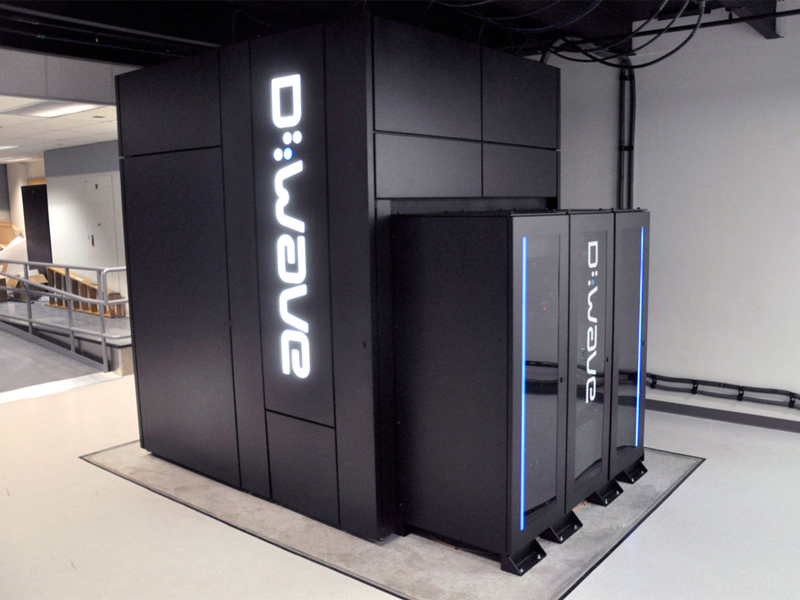
\includegraphics[width= .2\textwidth]{./images/quantum.jpg}
    \caption{``faux'' Ordinateur quantique D-wave}
  \end{figure}
  
  Cryptographie post-quantique candidates :

  \begin{itemize}
  \item Multi-variants
  \item Bas\'e sur les codes
  \item Bas\'e sur les r\'eseaux euclidiens (le seul qui peut fournir des arguments convaincants)
  \end{itemize}

\end{frame}


\begin{frame}{Th\`ese}
  \begin{itemize}
  \item Doctorant dans l'\'equipe EMSEC de l'IRISA \`a \\Universit\'e de Rennes 1. (Depuis 1er septembre 2016)
  \item Encadrant de th\`ese: Pierre-Alain Fouque, Adeline Langlois et Beno\^it Libert
  \item Sujet: Protocoles Cryptographique Post-quantique bas\'e sur le r\'eseau euclidien.
  \end{itemize}
\end{frame}
